\documentclass[]{report}
\usepackage{hyperref}
\usepackage{cleveref}
\usepackage{graphicx}
\usepackage{svg}
\usepackage{url}
\usepackage{minted}
\usepackage{dirtree}
\usepackage{fullpage}
\usepackage{etoc}

\setcounter{secnumdepth}{3}
% Title Page
\title{Local Computing Cluster Resources}
\author{Qimin Yan Group}


\begin{document}
\maketitle

\begin{abstract}
	This article gives an overview of the computational resources of our research group. Currently, it consists of several independent compute nodes, as well as one Slurm computational cluster. Basic usage is discussed along with the neccessary steps to set up new nodes and construct new clusters.
\end{abstract}

\tableofcontents

\chapter{Available Computational Clusters}

Currently, we have one operational cluster, which will be referred to as C1 (or simply `the cluster') hereafter. C1 consists of the basic tree network shown schematically in \cref{qyg-c1-schematic} with current IP addresses. The head node connects to both the internet (through ethernet port enp36s0f1) and the local cluster (port enp36s0f0).

The global IP address of the head node (enp36s0f1) is determined dynamically via DHCP by our network administrators and the local IP address (enp36s0f0) is set statically by us. All other IP addresses in the LAN are set statically. The local connection of the head node connects to the switch which acts as a central hub for all of the other network resources, namely the Network Attached Storage (NAS), and the compute nodes. 


\begin{figure}[h!]
	\centering
	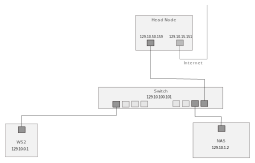
\includegraphics[scale=0.5]{qyg-c1-schem.pdf}
	\caption{A schematic detailing the basic tree architecture of C1.}\label{qyg-c1-schematic}
\end{figure}


The switch is a QNAP QSW-IM1200-8C and may be accessed and configured by connecting locally via an ethernet port and using the associated QNAP QFinder-Pro software. One may also access the switch by navigating to it's IP address in an internet browser on any locally connected device with an IP in it's subnet. To access the switch remotely, one can use SSH tunneling to forward the HTTP traffic to your local browser (see: \url{https://serverfault.com/questions/581530/https-ssh-tunnel}). This may be accomplished with the command:
\begin{verbatim}
	ssh -L 8443:<SwitchIP>:80 -Nf <user>@<HeadNodeIP>
\end{verbatim}
where HTTP traffic (port 80) from the switch is forwarded to localhost:8443 (open in your local browser) through the head node.

The NAS is an ASUSTOR which may be accessed and configured by connecting locally via an ethernet port and using the associated ASUSTOR Control Center software. One may also access the NAS by navigating to it's IP address in an internet browser on any locally connected device on it's subnet. If not in the subnet, one may forward the port 8000 to their localhost to access the ADM server. The NAS incorporates a redundant memory scheme to safely store data and is currently configured to the RAID 5 standard. Note that the NAS's OS is not Ubuntu but instead ASUSTOR Data Master (ADM), a proprietary OS. Many basic linux commands and packages are included and useable in it's terminal environment, however.

Compute nodes consist of PCs each with a single Intel i9 CPU and four Nvidia RTX 4090 GPUs. Each has Ubuntu installed as the OS.


\section{MAC Addresses for Static IP Addresses}
Static IP addresses may be requested from your ISP or local network administrator (in our case, the latter). Generally, the admin will require both the label of the ethernet port (in the wall) the device is connected to, as well as the MAC address of the ethernet port on the device (if there are multiple, the port connected to the wall/internet). For convenience, when making these requests, the MAC address of the relevant devices is given here, namely for the head node. Currently, the head node is connected to the internet via port \verb|enp36s0f1| with link/ether MAC address \verb|a8:a1:59:c7:0a:34|.

\begin{center}
\begin{tabular}{|c|c|c|}
\hline
Host Name & MAC Address & IP\\
\hline
MLWS1 &  c8:7f:54:c5:c9:63 & 129.10.14.227\\
MLWS2 & 08:bf:b8:03:56:c7 & 129.10.14.209\\
MLWS3 & 08:bf:b8:02:4d:e7 & 129.10.15.138\\
MLWS4 & 08:bf:b8:03:55:b7 & 129.10.14.210\\
HeadNode & a8:a1:59:c7:0a:34 & 129.10.15.158/50.159\\
DefectDB & b8:cb:29:f7:97:f5 & 129.10.14.\\
(old)WS1 & 58:11:22:9f:08:1f & 129.10.14.\\
\hline
\end{tabular}
\end{center}

Note that the relevant MAC addresses may change if the ethernet chord is plugged into a different port, since the MAC address technically refers here to the connected ethernet port.

 \chapter{Constructing a New Cluster}
 
 \etocsetnexttocdepth{1}
 \localtableofcontents
 
 \medskip
 
\noindent The construction of a new Slurm computational cluster consists of three basic steps: \textit{(1)} constructing a Local Access Network (LAN) and mounting the Network Attached Storage (NAS) across it; \textit{(2)} homogenizing users and software across nodes; and, \textit{(3)} installing Slurm and initializing it's daemons. For some research purposes, we also need to install OpenMX \textit{(4)}. Each of these basic steps are detailed in the following sections.

 \section{Local Access Networks}
A local access network (LAN) is a set of devices that are locally connected (often physically via ethernet cables) such that each may communicate without access to the internet. For a computational cluster, physical connections (cables) are almost always preferred to reduce network latency (time for communication between devices).

Constructing a LAN is relatively easy: first all devices must be locally connected (of course), and then each must be assigned an IP address on the same subnet. The IP address range for a subnet may be determined by some given IP address (often a global IP address which allows for internet connection and is determined by some ISP or IT staff) and a subnet mask.

The first division of digits of an IP determine it's class. The class of an IP address determines it's subnet mask, and corresponding number of devices it may have on it's subnet. We are often given some IP address from an ISP or network administrator which we may then build a subnet on. At Burlington, our IP range is in 129.10.x.x, so the netmask for all subnets is 255.255.0.0.

 \subsection{Configuring Gateway}
In the basic tree architecture used here, only the head node has direct connection to the internet. Thus, other devices in the LAN need to use the head node as a gateway to access the internet. This may be configured with iptables and route commands (from the \verb|net-tools| package). 

First pass this command on the local node to set the default gateway:
\begin{verbatim}
	sudo route add default gw 129.10.50.159
\end{verbatim}
Then, give the following on the gateway to allow forwarding and receiving on behalf of the subnet devices:
\begin{verbatim}
	 echo 1 > /proc/sys/net/ipv4/ip_forward
	 sudo iptables -t nat -A POSTROUTING -o enp36s0f1 -j MASQUERADE
	 sudo iptables -A FORWARD -i enp36s0f0 -o enp36s0f1 -j ACCEPT
	 sudo iptables -A FORWARD -i enp36s0f1 -o enp36s0f0  -m state --state RELATED,ESTABLISHED -j ACCEPT
\end{verbatim} 
Note that these commands require that the device (ethernet port) labeled enp36s0f0 is outward-facing (to the internet) and the device labeled enp36s0f1 is inward-facing; this simply means the device IDs given above need to be changed if the ethernet ports are changed.
See \url{https://unix.stackexchange.com/questions/222054/how-can-i-use-linux-as-a-gateway}. Note that
current networking routes may be checked with the \verb|routel| command.

Commands given by \verb|iptables| may not necessarily be persistent upon reboot (by default, no iptables commands will persist). To set persistent rules, first set the desired rules, then use \verb|iptables-save| and  \verb|iptables-restore| with the following command: 
\begin{verbatim}
	sudo iptables-save | sudo tee /etc/iptables.conf
\end{verbatim}
Then, to reload these rules automatically on restart, insert these lines into \verb|/etc/rc.local|:
\begin{verbatim}
	iptables-restore < /etc/iptables.conf
\end{verbatim}
See \hyperlink{https://askubuntu.com/questions/66890/how-can-i-make-a-specific-set-of-iptables-rules-permanent}{this askubuntu.com thread} for more detail.


 \subsection{Setting DNS Server on Subnodes}
A Domain Name System (DNS) is essentially a directory relating web addresses to IP addresses. For example, a DNS provides the map from the web address `www.google.com' to the IP address `8.8.8.8'. The head node has an IP address provided by our network administrator via a DHCP protocol that also provides a DNS server. 

Sub-nodes on the tree architecture used here may need to have their DNS servers updated or set manually, however. To set manually, see the file located at \verb|/etc/resolv.conf| and edit the IP address listed after \verb|nameserver|.
For more detail, see \url{https://www.geeksforgeeks.org/how-to-configure-dns-in-linux/}. One may also use a command, such as:
\begin{verbatim}
	echo "nameserver 8.8.8.8" | sudo tee /etc/resolv.conf > /dev/null
\end{verbatim}
However, this may not persist after startup for newer versions of Ubuntu.


To set a static DNS server on Ubuntu that doesn't get reset on restart, first install \verb|resolvconf| with \verb|apt|. Then, append a line containing the desired DNS server IP address after `nameserver' in  \verb|/etc/resolv.conf| or \verb|/etc/resolvconf/resolv.conf.d/head| and then run \verb|sudo service resolvconf restart|.  For more detail, see \url{https://datawookie.dev/blog/2018/10/dns-on-ubuntu/} or \url{https://anyware.hp.com/web-help/cas_manager/22.04/troubleshooting/dns_name_resolution/}. Note that 8.8.8.8 is Google's publicly available DNS server, and thus is a good choice due to it's reliability.

 \subsection{Installing Packages on Nodes Without Direct Internet Access}

In the basic tree architecture of C1, only the head node has direct internet access. This allows for the head node to act as a global firewall for the network but does hinder some functions of the compute nodes. The following introduces a set of commands that allows for packages to be installed using apt on offline devices through online repositories accessible by the head node.


From the device with internet access, first SSH into the local device without internet access with:
{\small
\begin{verbatim}
	ssh -R <selected port>:us.archive.ubuntu.com:80 user@nointernethost
\end{verbatim}}
We then need to create a file (if it doesn't already exist) '/etc/apt/apt.conf' and add the following two lines:
\begin{verbatim}
	Acquire::http::Proxy "http://localhost:<selected port>";
	Acquire::https::Proxy "https://localhost:<selected port>";
\end{verbatim}
Running apt on the remote node without internet access should then allow us to download packages as long as the former ssh command is active. In consequent uses, the configuration file should be maintained, so that only the first ssh command is needed.
This chain of commands is based on: \url{https://stackoverflow.com/questions/36353955/apt-get-install- via-tunnel-proxy-but-ssh-only-from-client-side}. 

 \subsection{Logging Into Subnode Via SSH Jumping}
For some inbound and outbound communications on subnodes without direct internet access, ip addresses must be jumped manually through the gateway. For example, this may be required to ssh into nodes off-LAN  with IPs in the LAN subnet. 
For \verb|ssh|, this is accomplished with the \verb|-J| option which requires an additional argument specifying the gateway node as:
\begin{verbatim}
	ssh -J <gateway-user>@<gateway-ip> <user>@<remote-ip>
\end{verbatim}
Similarly, to copy files with \verb|scp|:
\begin{verbatim}
	scp -J <gateway-user>@<gateway-ip> <file-to-copy> <user>@<remote-ip>:<remote-destination>
\end{verbatim}
See \url{ https://superuser.com/questions/456438/how-do-i-scp-a-file-through-an-intermediate-server}. Note that one may also update their ``$\sim$/.ssh/config" file to automatically jump for certain hosts with ProxyJump, as in \url{https://superuser.com/questions/174160/scp-over-a-proxy-with-one-command-from-local-machine}.



 \subsection{Mounting NAS}
The Network Attached Storage (NAS) is a cluster-wide storage node. For the NAS to be available on all other nodes, it must be automatically mounted at startup across the cluster. One popular way to do this for a hard-wired LAN is with NFS (see \url{https://help.ubuntu.com/community/SettingUpNFSHowTo}; note that another method must be used for wireless/WiFi-based clusters, such as autoFS, see \url{https://askubuntu.com/questions/884389/auto-mount-nfs-via-autonfs}). 

The NAS of C1 uses a proprietary linux-based OS that seems to require us to setup NFS access via an in-browser GUI. For these steps, see \url{https://www.asustor.com/en/online/College_topic?topic=109#lux3}.
Note that this browser applet on port 8000 for HTTP (8001 for HTTPS) may be accessed remotely with the command:
\begin{verbatim}
	ssh -L 9999:localhost:8000 -Nf <user>@<NAS-IP>
\end{verbatim}

The client-side nodes of the NAS then must all have the \verb|nfs-common| package installed (with \verb|apt| for instance). The shared directory on the NAS server then may be mounted on the clients with the following command:
\begin{verbatim}
	mount -t nfs <NAS-IP>:/<NAS-Shared-Folder> <Directory-to-Mount-to>
\end{verbatim}
This may be done automatically by appending a line of the following form to the file \verb|/etc/fstab|:
\begin{verbatim}
	<NAS-IP>:/<NAS-Shared-Folder>   <Directory-to-Mount-to>    nfs    defaults    0 0 :
\end{verbatim}
For more detail on how to update the \verb|fstab| file for automatic mounting at startup, see the following: \url{https://askubuntu.com/questions/890981/how-to-configure-a-nfs-mounting-in-fstab}. 
To test a newly updated \verb|fstab| file, the command \verb|mount -a| may be used to load it; however, this is apparently bad practice, and the command \verb|findmnt --verify| should be used first to verify the \verb|fstab| file isn't broken (as specified in \url{https://serverfault.com/questions/518967/do-i-need-to-restart-my-server-after-editing-fstab-and-mtab}).

Occasionally, NFS will return a 'stale file handle' error when trying to access mounted directories. In this case, try first unmounting with \verb|umount <mounted-dir>| and then remounting with \verb|mount -a|. For more detail on this issue, see \url{https://unix.stackexchange.com/questions/433051/mount-nfs-stale-file-handle-error-cannot-umount}.


 \section{Ansible}
To avoid manually installing a list of the same software and environments on each device of the cluster, software provisioning tools may be used to install cluster-wide in one command from one device. Many options exist, but here we consider Ansible, an open source IT automation engine that can be use to automate provisioning, and more generally the issuing of common commands across many devices simultaneously. A key concept in the design of Ansible is the distinction between \textit{state} and \textit{action}. An Ansible play is primarily supposed to describe a desired \textit{state} of a system, as opposed to a simple list of actions to perform. This is a particularly important point for provisioning across a cluster, since we generally desire just that all devices have certain packages \textit{installed} and opposed to a blind issuance to \textit{install} a set of packages. For a brief overview of some Ansible commands, see \url{https://spacelift.io/blog/ansible-cheat-sheet}.

Note that before using Ansible on remote devices, the current user must be able to SSH into the same remote devices without being prompted for a password. This may be accomplished by saving the SSH pair's public key, as shown in the following section (\ref{savesshkeys}). After this, an overview of the directory of current ansible playbooks for C1 is given; as well as a template for typical user downloads and conda environment tools.

 \subsection{Generating SSH Keys For Automatic (Password-less) Login}\label{savesshkeys}
If they do not already exist on the head node, first, generate RSA key pairs for  the head node's SSH client with the following command:
\begin{verbatim}
	ssh-keygen -t rsa
\end{verbatim}
Then, copy all necessary public keys into \verb|~/.ssh/authorized-keys| for each subnode using \verb|ssh-copy-id| with the following command (see \href{https://stackoverflow.com/questions/23591083/how-to-append-authorized-keys-on-the-remote-server-with-id-rsa-pub-key}{here}):
\begin{verbatim}
	ssh-copy-id <user>@<subnode-identifier>
\end{verbatim}
which will prompt you to log in as \verb|<user>| on the specified subnode. After this, no password should be requested in following ssh interactions (as current user on local device to \verb|<user>| on remote device, for each subnode this command was used on). This is a necessary prerequisite for every node Ansible is intended to run on.

 \subsection{Cluster Hosts}
The hosts available to Ansible are defined (by default) in the file \verb|/etc/ansible/hosts|, which requires sudo access to edit. Hosts may also be specified locally in a file \verb|inventory.ini| in the folder of ansible playbooks (see \href{https://docs.ansible.com/ansible/latest/getting_started/get_started_inventory.html#get-started-inventory}{here}).

\subsection{Available Playbooks}
Several playbooks are available in the related Github repository that may be used to automate the tasks outlined in the following subsections of this article: \nameref{slurmpre}, \nameref{slurmin}, \nameref{omxpre}, and \nameref{omxin}. 
These can be found in the \verb|ansible-playbooks| directory in a similar structure:

\medskip

\dirtree{.1 ansible-playbooks.
.2 slurm-setup.
.3 slurm-prerequisites.yml (\nameref{slurmpre}).
.3 install-slurm.yml (\nameref{slurmin}).
.2 openmx-setup.
.3 openmx-prerequisites.yml (\nameref{omxpre}).
.3 install-openmx.yml (\nameref{omxin}).
}

\section{Slurm}

 \etocsetnexttocdepth{3}
\localtableofcontents

\subsection{Prerequisites for Slurm Installation}\label{slurmpre}
A Slurm\footnote{SLURM is not an acronym...} cluster requires a homogeneous set of users and specific software across all nodes in the cluster. Specifically, the user names and user ids (UIDs) of the OS as well as the group names and ids (GIDs) must be the same across all the nodes. Furthermore, Slurm requires munge (a linux software package instantiating a set of secure communication protocols) be installed on each device,.which also requires a user named 'munge' on each device which must have it's ids synchronized. Finally, Slurm requires that the devices on the LAN all have synchronized clocks, which may be accomplished with ntp (another linux software package). In the following, we give detailed instructions for each of these processes.

 \subsubsection{Changing UIDs and GIDs}
The UIDs and GIDs can be found in the file '/etc/passwd' and changed with chmod commands. Users may be added with the useradd command. Note that the munge user id need not be synchronized between systems since it's a system user. 
For an article giving an overiew of the useradd command, see:
\url{https://linuxize.com/post/how-to-create-users-in-linux-using-the-useradd-command/}. If user accounts already exist and ids must be changed, the relevant commands are discussed \hyperlink{https://askubuntu.com/questions/16700/how-can-i-change-my-own-user-id}{here}.


\subsubsection*{Current UIDs and GIDs for Group Members}
Currently, we used the following set of UIDs for current (and past) members of the group:
\begin{verbatim}
#!/bin/bash
sudo useradd -m -u 1001 weiyi
sudo useradd -m -u 1002 ajh
sudo useradd -m -u 1003 anoj
sudo useradd -m -u 1004 yuboqi
sudo useradd -m -u 1005 tsai
sudo useradd -m -u 1006 zhenyaof
sudo useradd -m -u 1008 angush
sudo useradd -m -u 1009 ruanyu
sudo useradd -m -u 1500 slurm
\end{verbatim}
where we assume 'qimin' already exists as a sudo user with UID and GID 1000.

\subsubsection*{Change User Password}
To change a user's password, use the following command:
\begin{verbatim}
sudo passwd <username>
\end{verbatim}
which will prompt the current user to set the password for \verb|<username>|. See \url{https://askubuntu.com/questions/423942/change-password-on-root-user-and-user-account} for more detail.

\subsubsection*{Add User to Sudoers Group}
To grant a user sudo permissions, run the following command:
\begin{verbatim}
sudo adduser <username> sudo
\end{verbatim}
For more detail, see \hyperlink{https://askubuntu.com/questions/7477/how-can-i-add-a-user-as-a-new-sudoer-using-the-command-line}{here}.



 \subsubsection{Installing Munge}
Munge is a secure communication protocol that is use by Slurm to communicate between nodes in the cluster. 
Munge may be installed with apt with the following command:
\begin{verbatim}
	sudo apt install munge  libmunge2 libmunge-dev
\end{verbatim}
Note that we need to also install the lib and dev versions of munge, as in the command above, for Slurm to work properly.
 
After installation, it's daemon must be enabled to start automatically on startup with the following command on Ubuntu:


\begin{verbatim}
	sudo systemctl enable munge.service
	sudo systemctl start munge.service
\end{verbatim}
Then, install and initiate munge daemons on each compute node. The munge keys should be uniform across the cluster, this is done by copying the key '/etc/munge/munge.key' from the head node to each compute node and restarting the munge daemon.


\subsubsection*{Testing Munge Installation}
The munge status on a single node may be tested with the following command:
\begin{verbatim}
	munge -n | unmunge | grep STATUS
\end{verbatim}
The munge status between nodes may be tested from one node to another with the following command:
\begin{verbatim}
	munge -n | ssh <NODE_ADDRESS> unmunge
\end{verbatim}
For the official installation guide, see: \url{https://github.com/dun/munge/wiki/Installation-Guide}.

 \subsubsection{Synchronizing Clocks}
Synchronized clocks are particularly important for munge protocols, since they incorporate time stamps in credentials for finite length-of-time authentification.
Time synchronization is often achieved simply by installing the ntp package on linux with apt (or some other package manager).

Generally speaking, if ntp is installed on each device, and munge doesn't return an error communicating between devices, the clocks should be sufficiently synchronized.
 \subsection{Slurm Installation}\label{slurmin}                                                                      
To install Slurm, we then need to download the desired version of Slurm and then decompress and build it. Note that while Slurm packages exist on many linux repositories, none are (currently) directly supported by SchedMD (the company that manages Slurm). After compiling Slurm, a config file must be made specifically for the cluster, and loaded by Slurm. After configuration the Slurm daemons must be initialized and then Slurm commands should be available for scheduling and submitting jobs. Each of these steps is covered in more detail in the following.

 \subsubsection{Download and Compiling} 
The most current stable version of Slurm may be downloaded as a compressed tar-ball at:
\url{https://www.schedmd.com/download-slurm/}.
This tar-ball \verb|slurm.version.tar.bz2| may be decompressed with the following command:
\begin{verbatim}
	 tar -xf slurm.version.tar.bz2
\end{verbatim}
Then, change directory to the uncompressed source and execute \verb|./configure| with the appropriate options. An important argument here is \verb|--prefix=<install_dir>|, which allows us to specify the install directory of the slurm program. To aid in bookeeping of slurm builds, install with a prefix (as recommended \hyperlink{https://groups.google.com/g/slurm-users/c/9Qvs8q1Uc-A}{here}):
\begin{verbatim}
	sudo bash ./configure --prefix=\opt\slurm-<version_number>-build-<build_number>
\end{verbatim}
 After running the configure command, run the \verb|make| command in the same directory to compile the source and then execute \verb|make install|. If \verb|make install| returns an error of the sort "make: *** [Makefile:613: install-recursive] Error 1", try executing \verb|sudo make install-recursive| instead.


 \subsubsection{Configuring Slurm}
Manual configuration is particularly important for Slurm since every cluster is different and has a totality of hardware not local to any one node. The easiest way to create a new configuration file is to use the SchedMD endorsed html configuration tool which can be found at \url{https://slurm.schedmd.com/configurator.html}. Make sure the version number of the configurator matches the version of Slurm being installed.

The Slurm configurator returns a long list of text in the browser. This may be copied into a file 'slurm.conf' where Slurm will see it. On Ubuntu an appropriate location for this file is in '/etc/slurm' (which may need to be created if it doesn't already exist) if created with root access  or '/usr/local/etc' otherwise. This same configuration file must be on each node of the Slurm cluster.

 \subsubsection{Giving Slurm Access to Files}
By default, the Slurm user will be ineligible to read or write in directories it needs access to to perform logging, load configurations, etc. In this case we need to add these privileges to the 'slurm' user. On C1, the PID and log files are written in '/etc/slurm', with the following command being neccessary for the control node:
\begin{verbatim}
	sudo chown -R slurm:slurm /etc/slurm
	sudo chown -R slurm:slurm /var/spool/slurmctld
\end{verbatim}
Otherwise, for compute nodes:
\begin{verbatim}
	sudo chown -R slurm:slurm /etc/slurm
	sudo chown -R slurm:slurm /var/spool/slurmd
\end{verbatim}
To test run Slurm before starting the daemons, you can run it first on controller nodes with the command:
\begin{verbatim}
	slurmctld -D -vvvvvv
\end{verbatim}
and on compute nodes with the command:
\begin{verbatim}
	slurmd -D -vvvvvv
\end{verbatim}
where the -D option specifies we want outputs written to the terminal and the excessive number of v's indicates we want a very verbose output (useful for debugging). Note that slurmctld and slurmd may need to be run with sudo (at least) the first time to create certain files, etc. Note also that some directories may need to first be made manually with sudo and the mkdir command; such necessities are usually apparent from the errors returned when running the '* -D -v' commands above.

 \subsubsection{Starting Slurm Daemons}
If the only errors returned from the test runs above are failure to communicate between nodes, we now need to start the daemons for the Slurm control and compute functions.

Before we can start the daemons, we need to be sure the system daemon, systemd can see their service files, which can be accomplished by copying the service unit files to systemd's path directory on both control and all compute nodes as:
\begin{verbatim}
	sudo cp slurmd.service slurmctld.service slurmdbd.service /etc/systemd/system
	sudo cp slurmd.service slurmctld.service slurmdbd.service /etc/systemd/user
\end{verbatim}
After manually moving the daemons into systemctl's directory, we need to reload the daemon list with the command \verb|systemctl daemon-reload|. On the control node, we then need to enable the service on startup and start the service with the commands:
\begin{verbatim}
	systemctl enable slurmctld
	systemctl start slurmctld
\end{verbatim}
 On the compute node we perform, similarly
\begin{verbatim}
	systemctl enable slurmd
	systemctl start slurmd
\end{verbatim}
To check systemctl's status for the daemons, use the \verb|systemctl status <daemon-name>| command. Furthermore, \verb|stop| and \verb|restart| commands may also be passed with systemctl. 

 \subsubsection{Adding Slurm Commands to Path}
After manually installing slurm and starting it's daemons, we'd like to have the slurm commands in all users \$PATH, so that they may use the commands without specifying the install location as a prefix. This may be done by either appending the slurm install directory's bin and sbin subdirectories to the the Path as specified in \verb|\etc\environment| or by appending the lines \verb|$PATH = '<exe-dir>'| to \verb|\etc\profile|; see \url{https://askubuntu.com/questions/24937/how-do-i-set-path-variables-for-all-users-on-a-server}.

\subsection{Troubleshooting Slurm}

 \subsubsection{Checking Slurm Node Statuses}
The simple \verb|sinfo| will give a quick overview of the slurm cluster's status. For more info about a specific node, use the \verb|scontrol| command with the options:
\begin{verbatim}
	scontrol show node <node-name>
\end{verbatim}
which returns a more detailed status report. Also, consider checking the log file of the daemon, usually located at \verb|\var\log\<daemon-name>.log|.

 \subsubsection{Restarting Slurm Daemons (After Reboot)} 
Note that unscheduled reboots of the nodes will raise an error in their restarted daemons. In this instance, the \verb|scontrol show| command will return an error: ``Reason=Node unexpectedly rebooted". To fix this, first let all jobs complete in the queue, then with \verb|systemctl|, stop and restart the slurmd service. After this, issue the command:
\begin{verbatim}
	scontrol update NodeName=<node-name> state=resume
\end{verbatim}
on every affected node to resume it's availability for allocation. If \verb|state=resume| doesn't work, try \verb|state=idle|; for more detail see \url{https://www.reddit.com/r/HPC/comments/199yklr/slurm_logs_say_that_a_node_unexpectedly_rebooted/} or \url{https://stackoverflow.com/questions/57144602/restart-nodes-in-state-down}.

 \subsubsection{Invalid Node State Specified}
If a node refuses to go online and the error "Invalid Node State Specified" is raised, check the conflict between the configured setup and the hardware on the node. If the attribute \verb|ThreadsPerCore| is misaligned, nodes will not go online. In these cases, this line must be added to the \verb|slurm.conf| file or hyperthreading must be disabled in th BIOS of the worker node. See \url{https://lists.schedmd.com/pipermail/slurm-users/2020-April/005269.html}


\section{OpenMX}
\subsection{OpenMX Prerequisites}\label{omxpre}
OpenMX requires a few packages to be available on the device prior to it's installation. Some of these prequisite packages have prequisite packages of their own, summarized below in the following tree structure:

\begin{itemize}
	\item Intel OneAPI
	\begin{itemize}
		\item ifx
		\item icc
		\item icx
	\end{itemize}
	\item OpenMPI
	\begin{itemize}
		\item gfortran
	\end{itemize}
	\item ScaLAPACK
	\begin{itemize}
		\item BLAS
		\item LAPACK
	\end{itemize}
	\item FFTW

\end{itemize}
\subsubsection{Intel OneAPI}
For our devices, OpenMX 3.9.9 seems to be reliably \verb|make|'d with Intel OneAPI's compilers; namely: ICC (for C), ICX, and IFX (for FORTRAN). If these compilers are not already available on the device, they may be installed within the Intel oneAPI HPC Tookit.

\subsubsection*{Checking for OneAPI Compilers}

To verify that the Intel oneAPI compilers are correctly installed and accessible from the terminal, first ensure that the oneAPI environment has been initialized by sourcing the \texttt{setvars.sh} script located in \texttt{/opt/intel/oneapi/}. Once the environment is active, you can check for the availability of specific compilers by running commands: \verb|ifx --version| for the Intel Fortran compiler and \verb|icx --version| for the Intel C/C++ compiler. If these commands return version information instead of a ``command not found'' error, the compilers are properly configured and ready for use. 

\subsubsection*{Installing Intel OneAPI HPC Toolkit}
To install the oneAPI HPC-toolkit with apt, which includes all the necessary compilers for building OpenMX, you first need to manually add Intel's oneAPI repository mirror to apt's mirror list, and then install with \verb|apt|.

\subsubsection*{Adding the Intel GPG Key}
Use the package \verb|gnupg|
Intel signs its software with a cryptographic GPG key to guarantee the authenticity of its packages. 
By downloading and importing this public key into the local keyring, the system gains the ability to verify that any Intel package originates from a trusted source and has not been modified in transit. 
This step is fundamental for maintaining the security of the software installation process.

\subsubsection*{Configuring the Intel oneAPI Repository}
To access Intel’s software through the package manager, a repository configuration file is added to the system under \verb|/etc/apt/sources.list.d/|. 
This file contains a reference to Intel’s official oneAPI repository, enabling the operating system to locate and install Intel software packages directly using standard APT commands. 

\subsubsection*{Refreshing the Package Index}
After introducing a new software repository, the package index must be refreshed using \verb|apt update|. 
This command synchronizes the local list of available software with all configured repositories, ensuring that the system is aware of the new Intel mirror before installation begins. 

\subsubsection*{Installing HPC Toolkit}
The Intel oneAPI HPC Toolkit can then be installed directly with  \verb|sudo apt install intel-oneapi-hpc-toolkit|.

\subsubsection{OpenMPI}
OpenMPI, and it's dependencies can luckily be installed directly using apt as follows:
\begin{verbatim}
	sudo apt install openmpi-bin libopenmpi-dev gfortran
\end{verbatim}
These should be installed first so that the ScaLAPACK can see the available MPI binaries.

\subsubsection{ScaLAPACK}
ScaLAPACK can be installed from the associated \verb|.tgz| file from \url{https://github.com/Reference-ScaLAPACK/scalapack/archive/refs/tags/v2.2.2.tar.gz}. For more detail on installation of ScaLAPACK see \hyperlink{https://www.netlib.org/scalapack/lawn93/node3.html}{here} or the document found at \url{http://www.netlib.org/scalapack/scalapack_install.ps}.

\subsubsection{FFTW}
FFTW can be installed by downloading the associated \verb|tgz| file from \url{} and following the usual \verb|./configure|, \verb|make|, \verb|make install| chain.

 \subsection{OpenMX Installation}\label{omxin}
OpenMX is a software package that can calculate self-consistent field equations for atomic arrangements in a real-space electron orbital basis. It can be installed manually in the usual manner, by downloading it's compressed source file, then uncompressing and \verb|make|-ing it, though you often need to play with it's \verb|makefile| since the usual configure script is not available. Here, we use Intel oneAPI compilers compatible with OpenMPI by including the lines in this makefile:
\begin{verbatim}
sMKLROOT = /opt/intel/oneapi/mkl/2025.3
CC = mpiicx -O3 -xHOST -fiopenmp -fcommon -Wimplicit-function-declaration -Wno-error=implicit-int -Wno-error=implicit-function-declaration -I${MKLROOT}/include -I${MKLROOT}/include/fftw
FC = mpiifx -O3 -xHOST -fiopenmp
LIB= -L${MKLROOT}/lib/intel64 -lmkl_scalapack_lp64 -lmkl_intel_lp64 -lmkl_intel_thread -lmkl_core -lmkl_blacs_openmpi_lp64 -lmpi_usempif08 -lmpi_usempi_ignore_tkr -lmpi_mpifh -liomp5 -lpthread -lm -ldl
\end{verbatim}
Note again, that these compilers are only available after \verb|source|-ing (for \verb|bash| or \verb|.| for \verb|sh|) the environment shell script \verb|/opt/intel/oneapi/<version>/oneapi-vars.sh|.


 \chapter{Basic Usage}
This section details basis usage of the cluster, namely the submission of jobs to the scheduler through Slurm, and the execution of cluster-wide commands through Ansible.

 \section{Submitting Jobs (Slurm)}
Slurm jobs may be run across the cluster by submitting \verb|sbatch| commands or directly with \verb|srun| commands. 

 \subsection{Interactive Shell on Slurm}
To be granted an interactive bash shell on the cluster, run the command:
\begin{verbatim}
	srun --pty bash -i
\end{verbatim}


 \section{Cluster-wide Commands \& Installation (Ansible)}
Ansible runs \textit{playbooks} on sets of nodes specified in YAML files.

\subsubsection*{Installing Packages Cluster-wide}
First, and perhaps most commonly, we generally install packages cluster-wide with the following playbook:
\begin{verbatim}
	---
	- hosts: all
	  tasks:
	  - name: install packages
	    become: true
	    become_user: root
	    apt:
	      state: present
	      name:
	      - python
	      - conda
\end{verbatim}
See \url{https://opensource.com/article/20/9/install-packages-ansible}.
Note that for tasks that require root privileges (such as the example above with \verb|become_user: root|), the option \verb|--ask-become-pass| must be passed as:
\begin{verbatim}
	ansible-playbook --ask-become-pass ./playbook.yml
\end{verbatim}
For generic shell commands across the cluster using ansible, see \url{https://kodekloud.com/blog/ansible-shell-module/}.See \url{https://opensource.com/article/20/9/install-packages-ansible}.
\end{document}          
